\documentclass[../main.tex]{subfiles}

\begin{document}
In questo capitolo si descrive la progettazione e lo sviluppo di una riproduzione del famoso gioco Snake adottando il paradigma Functional Reactive Programming. Al requisito non funzionale dell'utilizzo del paradigma FRP e del linguaggio di programmazione Scala si aggiunge anche quello dell'utilizzo della libreria \textit{Sodium}, analizzata nel capitolo precedente e scelta per la chiarezza e la completezza (ovvero il rispetto del paradigma FRP) delle API fornite.

I requisiti funzionali della applicazione \textit{FRP Snake} sono:
\begin{itemize}
    \item Il serpente si muove di una posizione nelle direzioni su, giu, destra e sinistra ed ha una dimensione iniziale pari a 1.
    \item Il numero di elementi che il serpente può mangiare è costante durante tutta la durata del gioco: quando il serpente mangia un elemento deve essere aggiunto un nuovo elemento.
    \item Gli elementi che il serpente può mangiare sono di due tipi: "buono", aumenta il punteggio complessivo di 100 punti e "cattivo", diminuisce il punteggio complessivo di 100 punti. In entrambi i casi il serpente aumenta la sua dimensione di 1 unità.
    \item La velocità di movimento del serpente è settata a 1 unità al secondo e può essere modificata a runtime in qualunque momento.
    \item Una partita si conclude quando il serpente è annodato.
\end{itemize}

\section{Progettazione}

\subsection{Input e Output}
Il seguente diagramma rappresenta gli input e gli output dell'applicazione in relazione agli elementi della GUI:
\begin{description}
  \item[directionInput] - Gli eventi associati alla pressione dei tasti "freccia su" (\textit{VK\_UP}), "freccia giu" (\textit{VK\_DOWN}), "freccia destra" (\textit{VK\_RIGHT}) e "freccia sinistra" (\textit{VK\_LEFT}) modificano il valore dell'input \textit{directionInput}, utilizzato per computare il movimento del serpente.
  \item[statusInput] - Gli eventi associati alla pressione dei tasti "S" (\textit{VK\_S}), "Q" (\textit{VK\_Q}) e "P" (\textit{VK\_P}) modificano il valore dell'input \textit{statusInput}, utilizzato rispettivamente per avviare/riprendere, terminare o sospendere la partita in corso.
  \item[speedInput] - Gli eventi associati alla pressione dei tasti "U" (\textit{VK\_U}) e "D" (\textit{VK\_D}) modificano il valore dell'input \textit{speedInput}, utilizzato per computare la velocità di movimento del serpente (frequenza dell'engine di gioco).
  \item[snakeOutput] - Stream attivato ogni volta che viene modificato il corpo del serpente, in seguito al movimento o all'eliminazione di un elemento "cibo".
  \item[foodOutput] - Stream attivato ogni volta che viene modificato l'insieme degli elementi "cibo" presenti nel mondo di gioco.
  \item[scoreOutput] - Stream attivato ogni volta che viene modificato il punteggio, ovvero quando viene eliminato un elemento "cibo" e quindi aumentata la dimensione del corpo del serpente.
\end{description}

\begin{figure}[H]
\centering
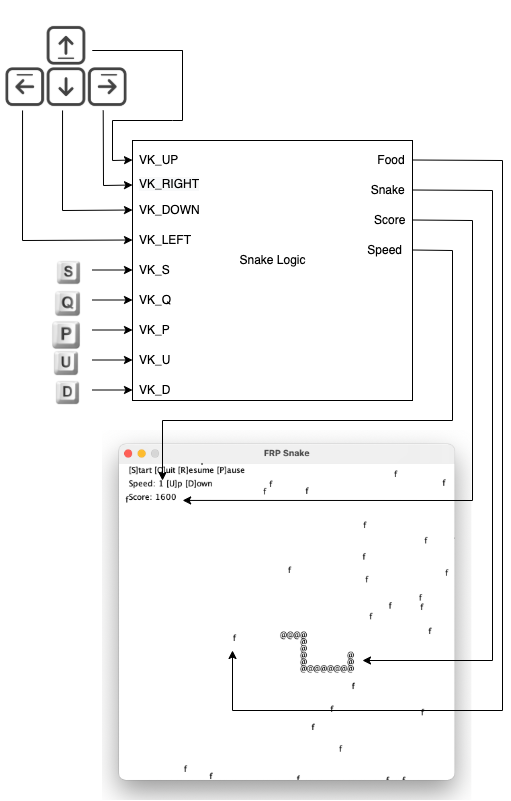
\includegraphics[width=0.9\textwidth]{img/frp-scala-Page-2.drawio.png}
\caption{Input/Output del programma FRP in relazione alla GUI}
\end{figure}

\newpage
Data la definizione in termini FRP degli input e output della applicazione, il seguente diagramma rappresenta il diagramma delle dipendenze che permette all'engine FRP di computare gli output alla modifica dei valori in input:
\begin{figure}[H]
\centering
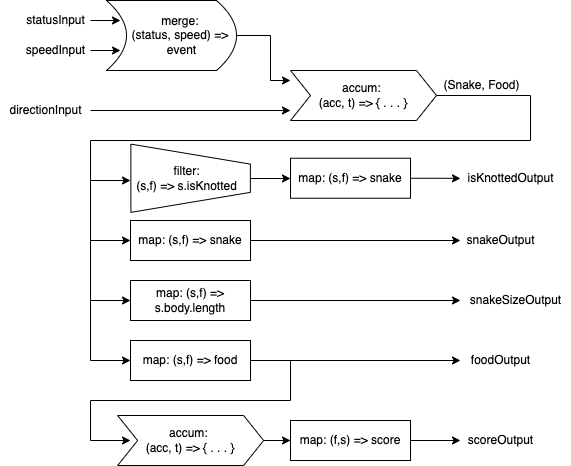
\includegraphics[width=0.9\textwidth]{img/frp-scala-Page-5.drawio.png}
\caption{Grafo delle dipendenze: FRP Snake}
\end{figure}
\end{document}

\section{Implementazione}
